%----------------------------------------------------------------------------
\renewcommand{\thechapter}{\Alph{chapter}}
\chapter*{Introduction}\addcontentsline{toc}{chapter}{Introduction}\label{chap:introduction}\setcounter{chapter}{9} 
%----------------------------------------------------------------------------
\section{Traffic load estimation}
%----------------------------------------------------------------------------
In recent years, there has been an increased scope for the automatic analysis of urban traffic activity\cite{Buch2011}.
This case is due to the increasing number of vehicles, the need for better understanding traffic dynamics for investment purposes, and also the accessibility of various sensors.
Formerly traffic estimation was performed by operators, by the means of on-the-spot observation or video analysis.
The main concept of traffic analysis is to aid or fully avoid human operators by automating these processes.

The information obtained by traffic monitoring systems are widely used to regulate traffic flow and contribute to administrative decisions about transportation infrastructure development, maintenance and investments \cite{MagyarKozut}.
In addition to the detection and classification of road users, that is an elementary task, several other monitoring objectives can be supported. 
Typical traffic data such as flow, density, and average speed can be extracted.
Some systems also recognize various situations including traffic violations or accidents (e.g., cars, motorbikes, and pedestrians).
Other real-time applications notify users about congestions, roadworks and accidents, or control traffic lights in order to influence traffic flow intensity in one direction \cite{AzoSensor, Thiruverahan2015, Ghazal2016}.
It is also possible to estimate environmental measures such as greenhouse gases, pollutant emissions, and fuel consumption in real time using high-resolution video traffic data combined with instantaneous emission models\cite{Morris2012a}. 
In the long term surveillance systems will be integral parts of the smart city infrastructure, modelling, identifying and influencing these city's traffic dynamics\cite{SOLSUN}.

\subsection{Traffic monitoring techniques}
Nowadays a variety of sensing modalities is available for on-road vehicle detection.

Inductive loop systems installed in the road are considered the most reliable traffic classification and detection method available, since larger metal objects can be accurately detected this way. 
On the other hand, the installation and maintenance is time-consuming and difficult, and slow or temporarily stopped vehicles cannot be detected\cite{Diamond, Zhang2016}.

Other active detection methods, including radar \cite{DeepBlue}, infrared\cite{Swarco, Hussain1995, Ghazal2016} and laser\cite{SICK, Gallego2009} sensors, are also popular owing to their robustness, although a complex machinery needs to be deployed.

Weight-based classification and speed detection is also possible using a piezoelectric sensor\cite{Te, Rivas2017}.

Video cameras have been installed for a long time for traffic monitoring purposes, because they provide a rich information source for human understanding with a relatively low cost of deployment\cite{Tian2011, Buch2011, VideoSurveillance, LaSemaforica}.
Nowadays cameras became even cheaper, smaller, and of higher quality than ever before, and vision-based surveillance is becoming the most popular form of vehicle detection.
In contradistinction to active sensors, cameras provide a wide field of view, allowing for detection across multiple lanes. 
Vision also integrates well with active sensor suites\cite{Garcia2012}.
The drawbacks to vision-based vehicle detection include sensitivity to light and weather conditions and increased computational cost\cite{Sivaraman2013}.

Multi-modal suites use sensor fusion to combine the data that results from the approaches outlined above\cite{Swarco}.

\subsubsection{Real-time vision sensors}
Although most vision sensor networks use a digital backend system where the captured data is transferred, and computation and storage takes place, since computing power has dramatically increased in the recent years, a new generation of visual surveillance systems has emerged.
These embedded sensors are capable of on-board high-level video processing with limited resources for computation, memory and power \cite{Bramberger2004}.
These platforms have the ability to reliably detect and track on-road vehicles in real time, since they utilize the new image-processing paradigms and advanced hardware: parallelization, multi-core processing and graphical processing units (GPUs)\cite{Sivaraman2013}.
Although the embedded platforms can provide sufficient computing performance, efficiently developing and porting software for these platforms is still a difficult and tedious task\cite{Bramberger2004}.
In this thesis an efficient traffic estimation method for embedded hardware is proposed, that can operate in real time for extended periods.
The implementation and realization details are discussed in the following chapters.

\subsection{Some results in video-based traffic monitoring}
In this section approaches in video-based on-road traffic monitoring are discussed, in particular with regard to techniques used in monocular vision.

Even though very diverse solutions has been suggested in the literature for vision-based surveillance problems, these methods are similar in the fact that they utilize the high information-content of the video stream, whilst the useless data are being identified and omitted for speed purposes.

Most vehicle counting methods are composed of three levels of perception built upon each other: detection, tracking and behaviour understanding.
The two upper levels use information extracted from the lower ones, since vehicles are continuously detected across several frames for tracking purposes, and behaviour understanding relies strongly on the trajectory of the object.

At the first level, the goal is to tell vehicles apart from the background using distinctive features: appearance or motion.

On of the two main approaches is appearance-based selection, wherein basic image characteristics such as colour\cite{Chang2005}, edges\cite{Blanc2007}, symmetry\cite{Aytekin2010}, HOG\cite{Niknejad2012}, Haar-like\cite{Sivaraman2012}, Gabor\cite{Zhang2006}, SIFT\cite{Zhang2011} or SURF\cite{Lin2012} features are used to identify vehicles.
In recent years, there has been a transition from simpler image features like edges and symmetry to general and robust feature sets\cite{Sivaraman2012}.
These detection methods are both applicable for moving and stationary objects or cameras, but require prior information about foreground object appearances.

These extracted features along with others are widely used for vehicle classification.
Most common distinctive attributes are heigh and length\cite{Huang2004}, linearity feature -- meaning the roughness of the vehicle contour\cite{Zhang2008} --, convex hull of the silhouette\cite{Buch2010} and distance between contour points\cite{Lou2005}.
Well-known descriptors like SIFT\cite{Zhang2011}, SURF\cite{Lin2012}, HOG\cite{Niknejad2012} and a handful of others are also popular.
Automatic license plate recognition, that is also extensively used, relies on these features\cite{Luvizon2016}. 

Classifiers can be broadly split into two categories: the less popular discriminative classifiers, that learn the underlying distribution of a given class; and generative ones relying upon hard decision boundaries between classes\cite{Sivaraman2012}.
Discriminative methods include artificial neural network classifiers\cite{Xia2006}, support vector machines\cite{Cornelis2008}, k-nearest neighbour (kNN) classifier\cite{Morris2006}, and AdaBoost\cite{Khammari2005}.
Popular generative classifiers are hidden Markov models\cite{Jazayeri2011}, probabilistically weighted vote\cite{Lin2012}, and hidden random field\cite{Zhang2011}.

Motion-based vehicle detection has been less common than appearance-based methods.
The core idea is to separate moving foreground from motionless background.
This approach relies on background subtraction: the static scene is estimated with various models and moving object are separated accordingly.
Several filters have been proposed for background subtraction, including frame differencing\cite{Park2007}, averaging\cite{Kanhere2008}, graph cuts\cite{Woodford2009}, as well as more sophisticated background models, such as Single Gaussian\cite{Kumar2003}, mode estimation\cite{Zheng2006}, Kalman-filter\cite{Messelodi2005} or wavelets\cite{Gao2009}. 

One of the most common subtraction techniques is Gaussian Mixture Modelling(GMM)\cite{Niknejad2012, Wang2009,Zhang2016a}, wherein each pixel is temporally modelled as a mixture of two or more Gaussians and is updated online\cite{Stauffer1999,Stauffer2000}.
GMM is considered one of the best parametric background models that are widely used, owing to its robustness and effectiveness over different scenes\cite{Zhang2016}.
Although most subtraction techniques assume a fixed scene, GMM can deal with both stationery backgrounds and repetitive changes in light.
The implementation in \cite{Kaewtrakulpong2001} is available in the OpenCV library and is commonly used in research\cite{OpenCVMog2}.

One level up dynamic parameters are measured and the position of road-users is approximated using various tracking algorithms. 
The main purposes of following vehicles across frames is to estimate  motion, predict vehicle positions, and enforce temporal coherence to omit false positives in counting.
Tracking algorithms range from simplest -- like geometric constraints\cite{Rabe2007}, optical flow\cite{Bhaskar2015}, template matching\cite{Liu2007}, feature-based tracking\cite{Haselhoff2009} -- to most complex, including particle filtering\cite{Danescu2011}, Kalman-filter\cite{Bresson2015}, spatial-temporal Markov random field (S-T MRF)\cite{Zhu2005}, graph correspondence\cite{Lai2010} and event cones\cite{Andrienko2015} along with others. 

The highest level of semantic interpretation lies in characterizing the behaviour of vehicles on the road\cite{Sivaraman2013}.
An aggregate of spatio-temporal features is used to learn, model, classify, and predict the behaviour and goals of other vehicles on the road.
Certain studies categorize observed vehicle behaviour as normal or critical\cite{Cherng2009}, others identify specific maneuvers, like lane changing or turning\cite{Garcia2012}, some works try to forecast vehicle trajectory using trajectory-based predictors\cite{Hermes2009}, others focus on incident detection\cite{Kamijo2004}.
Maneuver-classification methods include hidden Markov model\cite{Sivaraman2011}, Bayesian networks\cite{Kasper2012} as well as Gaussian mixture modeling\cite{Wiest2012}.

Handling extreme weather or light conditions is always challenging for visual sensors, therefore a series of different solutions has been proposed to be able to process scenes with rain\cite{Yu2015,Barnum2010}, thick fog\cite{Zhou2014a,Tarel2009}, night-time\cite{Bi2009, Robert2009} or heavy shadows\cite{Kamkar2016, Miller2015}.

\subsubsection{Counting vehicles with time-spatial images}
Many traditional methods fail in real-time, embedded environments for traffic counting purposes, due to their high computational complexity.
Hence one of the challenges of real-time traffic monitoring is to decrease the aforementioned computation time by minimizing the information processed by filtering the image domain.

The selection of relevant information often relies on a priori knowledge of the scene, including direction of traffic flow and assumed trajectory of bypassing vehicles.
Many of these selection techniques restrict the calculation to an interested region in the traffic scene, e.g. virtual loops\cite{Tursun2013a, He2008} or detection regions\cite{Miller2015, Engel2016} placed in the way of vehicles.

\begin{figure}[!h]
	\centering
	\includesvg[width=0.9\textwidth]{original_frame_timeline.svg}
	\caption{Virtual detection line in a frame (left), and a time-spatial image created from the original frame sequence (right).\label{fig:TSI}}
\end{figure}

One of the most cost-effective, image-domain reducing techniques is based on virtual detection lines (VDLs) and time-spatial images (TSIs).
A virtual detection line is a one-pixel wide straight line placed perpendicular or parallel to the vehicle trajectory, whilst a time-spatial image can be considered itself as an image, where the vertical dimension corresponds to the VDL in the original frame, and the horizontal one corresponds to time in the original sequence.
A time-spatial image reflects the state of a fixed line changes with time, thus if a vehicle crosses or touches the VDL, it appears in the TSI and becomes detectable, as seen in figure \ref{fig:TSI}.
Such images can also be perceived as a sequence from a line-detector, or the cross-section of the traffic flow that condenses essential information. 

An approach similar to the aforementioned was first introduced in 2001 by Albiol et. al., and was proposed for counting people in video sequences using a "stack of lines" -- that is the equivalent of a TSI\cite{Albiol2001}.

An approach with virtual line groups placed both perpendicular and parallel to the traffic flow direction was proposed later for counting\cite{Anan2006,Wu2007}.

A background subtraction method based on frame differencing was used in \cite{Anan2006, Wu2007}, wherein background estimation and detection took place solely on the VDLs.
This has the advantages of high operation speed and strong real-time ability, due to processing only a rather small portion of the image, however this method is unable to measure vehicle length and other distinctive features necessary for classification.

In 2008 Li et. al. proposed a time-spatial imagery based algorithm to analyse congestions on urban roads.
Li used perpendicular lines to detect and count vehicles in normal traffic flow, and parallel lines to identify a congestion scene\cite{Li2008}.

Yue evaluated traffic-flow parameters under urban road environment with the same method\cite{Yue2009}.

A similar technique was also introduced by Rashid et. al., wherein vehicles were detected and counted on a TSI, and feature-based classification was performed using attributes like width, area and rectangularity extracted from both the TSI and frames\cite{Rashid2010}.

Mithun et. al. proposes a kNN classification scheme using shape-based, shape-invariant, and texture-based features of the segmented regions corresponding to the vehicles in the TSIs\cite{Mithun2012a}.

Both Yue, Rashid and Mithn uses an appearance-based detection method, since TSIs are extracted from the original video sequence without background subtraction performed, and vehicles are identified using an edge detector.

In 2013 Yang et. al. discussed a new approach for time-spatial imagery extraction\cite{Yang2013a}.
Their motion-based method includes background subtraction and feature extraction (colour and edge invariants) on each frame before the TSI is created.
The resulting foreground- and feature-TSIs were used to detect vehicles, eliminate shadows and manage occlusions.
Yang also evaluated several traffic flow parameters, including velocity, flow, road occupancy and density by measurements carried out on the original frames. 
Vehicle length and region size was used to classify vehicles.

Kryjak et. al.'s concept is based on detecting the presence of vehicles by analysing only the local neighbourhood of a VDL.
Kryjak also implemented the method in real-time for an embedded hardware\cite{Kryjak2014}.

In a recent study by Kamkar et. al. TSIs are generated to measure vehicle length. Vehicles are classified using a pre-trained random forest classifier\cite{Kamkar2016}. 
Kamkar's approach analyses both the time-spatial domain, and corresponding regions in the original frames to extract classifying features.
Note that in this study TSIs are used solely for classification purposes, the detection is performed on the original images.

On of the latest studies on this topic is Zhang's, in which a foreground time-spatial image (FTSI) is proposed for counting vehicles in complex urban traffic scenes\cite{Zhang2016}.
In this study a self-adaptive sample consensus background model is created, and foreground is estimated only on the VDL.
Occlusion are filtered using the convexity of the objects of the FTSI.

As the above examples show, TSI approaches are often implemented for real-time monitoring due to its low computational cost.
It can be realized as a part of an intelligent transportation system owing to its ability to function under a wide range of traffic situations, like occlusion, dense traffic, slow or temporarily stopped vehicles; and also a variety of lighting conditions, including sunny weather, night, rain, twilight, etc.

Drawback to using a TSI-based method for detection purposes is that the analysis on the time-spatial imagery is one-dimensional, making it impossible to measure and extract data perpendicular to the detection line.
Therefore most systems utilize a combination of frame-based and TSI-based features for classification purposes and for making the counting more accurate, as seen in \cite{Kryjak2014, Yang2013a}. 
Although this approach moderately slows down the processing, it opens a wide range of other possible applications, including occlusion detection and traffic flow parameter evaluation.
%----------------------------------------------------------------------------

\section{The SOLSUN project}
The intelligent transportation system detailed in this work has been developed as a sub-project of the SOLSUN (Sustainable Outdoor Lighting \& Sensory Urban Networks) international project\cite{SOLSUN}.
The goal of the SOLSUN project is to deploy an intelligent sensor network installed within existing street lighting to monitor the urban environment.
Each node of the network is a street light lamp containing a complex sensor suite made up by several sensors, capable of monitoring both emission, noise pollution, weather and traffic density at the same time.
The data collected by these nodes gets transferred to a central backend system through a communications network to be interpreted.
Information gathered will be used to reduce energy consumption by increasing cost-effectiveness of the street lights.
Traffic flow data will contribute to management and planning of traffic dynamics of the monitored region and thus reducing the emission of greenhouse gases as well.
SOLSUN supports the objective of demonstrating how an intelligent city infrastructure can be created in a cost-effective and sustainable way.

%----------------------------------------------------------------------------
\subsection{Goals and constraints of the SOLSUN Traffic Sensor sub-project}
The sub-project dedicated to the traffic sensor as part of the SOLSUN system, started in 2015 at the Department of Automation and Applied Informatics at BME\cite{SOLSUN_BME}.
The goal of the sub-project is to device a conceptional prototype software system for traffic monitoring purposes, that is able to function in real-time in an embedded environment.
The done product is stable enough to work for extended periods of time in the production environment for further testing and improvement.

The primary task of the application is traffic flow estimation, that is performed by counting the recorded vehicles with a 70\% error-rate at least.
Secondary aim is classification: the vehicles may be categorized into five types, namely car, cyclist, truck, pedestrian and other.
The categorization is important, hence it contributes to emission-estimation when data is interpreted at the centre\cite{Csorba2016}.
Other features, like speed and following distance estimation should be supported as well.

Real-time requirements imply that the processing speed exceeds \SI{25}{frame/s}, as under this speed the risk of missing frames, thus missing vehicles as well is reasonably high.

The traffic sensor application will run on its own built-in core integrated into the sensor suite.
The hardware itself must be able to function with passive cooling due to the embedded environment: SOLSUN sensor system will be installed inside a street-lighting lamp box.

Traffic monitoring is done by a camera sensor, that connects to the board through a USB port.
The complete video processing takes place on the board, and the resulted data, including vehicle count and type, speed, and following distance, is transferred to the backend through a communications network in a compact file format.
The communication is managed through the EnTalk\textsuperscript{TM} network, the hardware manufacturer's own data channel and remote street light management system\cite{EnTalk}.

Since surveillance is performed from a street-lighting lamp, from the side of the road, the camera's focal axis is vertical.
To record the complete width of the road from this position and angle, a camera with wide field of view (e.g. a panoramic one) is essential.
Moreover, the precise position of the camera is varying based on the particular setting where the sensor is placed, thus a robust application supporting slightly heterogeneous conditions and surroundings needs to be deployed. 
An example of the view is depicted in figure \ref{fig:camera_position}.
Additionally, the application needs to operate through extended periods of time with changing light, weather and traffic conditions, increasing the need for the robustness of the detection method.

\begin{figure}
	\centering
	\begin{subfigure}[b]{.5\textwidth}
		\centering
		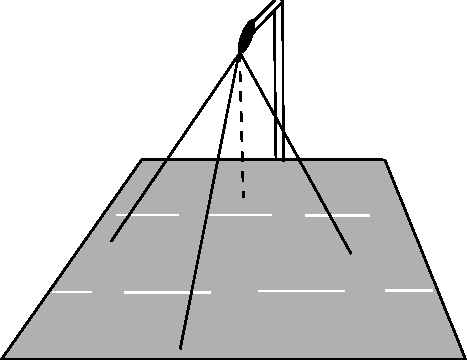
\includegraphics[width=0.9\linewidth]{kamera_placement.pdf}
		%\caption{A subfigure}
		%\label{fig:sub1}
	\end{subfigure}%
	\begin{subfigure}[b]{.5\textwidth}
		\centering
		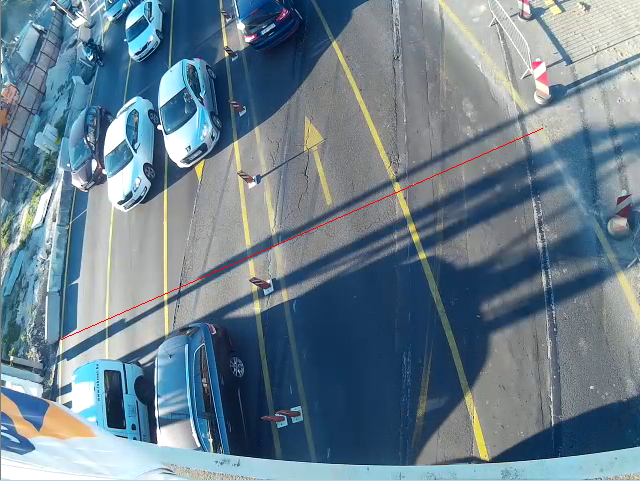
\includegraphics[width=0.8\linewidth]{raw_frame_perspective.png}
		%\caption{A subfigure}
		%\label{fig:sub2}
	\end{subfigure}
	\caption{Camera placement and a typical frame scene of the Traffic Sensor. The camera's optical axis is vertical. To monitor the entire width of the road a panoramic camera with a wide angle of view was used for testing purposes.}
	\label{fig:camera_position}
\end{figure}

The criteria detailed above, including the robustness of the application, the requirement of passive cooling -- that limits hardware performance --, alongside with the demand of real-time operation, generate strict specifications for the software itself.
Therefore whilst developing the system framework, our team's goal was to combine computationally effective, real-time video processing algorithms and software engineering paradigms in order to create an efficient product satisfying all of the above requirements.

The application was implemented in C++ with QT framework.
For image processing tasks some algorithms from the OpenCV (Open Source Computer Vision Library) were used.

\subsection{Contribution of this thesis}

I have been working on the Traffic Sensor sub-project since the start, developing and implementing video processing methods and algorithms, and designing the architecture of the application.
Although the results and methods discussed in this thesis are product of the collective work of the project team, some particular solutions are my own. 
Even though my own contributions are emphasized throughout the thesis, to fully understand the operation and architecture of the application, the entire product is outlined in this work.

%----------------------------------------------------------------------------
\section{Thesis goals and organization}
%----------------------------------------------------------------------------
In this thesis the operation and structure of the Solsun Traffic Sensor is detailed, in particular with regard to the core software architecture, the hardware environment, network organization and supplementary software elements.
The work focuses on the results of the performance tests and software experiments, as well as further improvement propositions.

The thesis is structured as follows.

The \ref{chap:Concepts}.~chapter introduces some basic terms and concepts essential for understanding the operation of the Traffic Sensor. 
The \ref{chap:Core software}.~chapter presents the structure of the core software side by side with the video processing steps.
In chapter \ref{chap:Environment}.~the supplementary software and hardware elements linking the system together are detailed.
The \ref{chap:Tests}.~chapter describes the results of the hardware and software experiments, discusses prevalent error impacts, and proposes related methods to improve the detection rate.
